\begin{figure}[ht]
\centering

\begin{subfigure}[b]{0.45\textwidth}
    \centering
    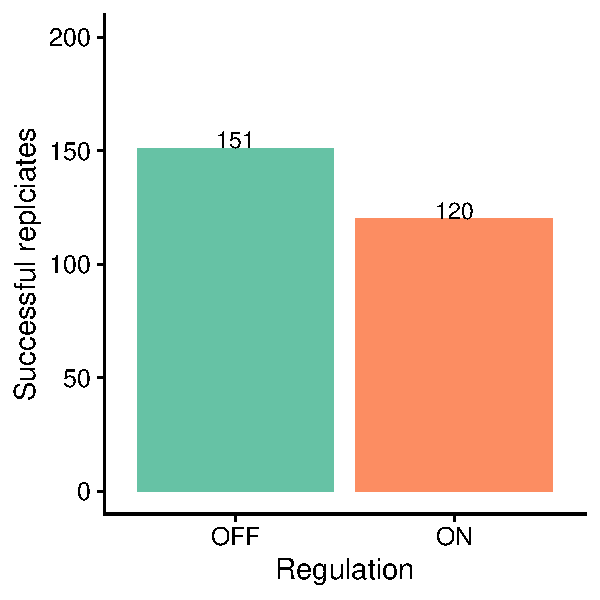
\includegraphics[width=\linewidth]{chapters/05-tag-based-genetic-regulation/media/boolean-calc-postfix-solution-counts.pdf}
    \caption{\small Successful replicates.}
    \label{chapter:tag-based-regulation:subfig:boolean-calc-postfix-solution-count}
\end{subfigure}
\hfill
\begin{subfigure}[b]{0.45\textwidth}
    \centering
    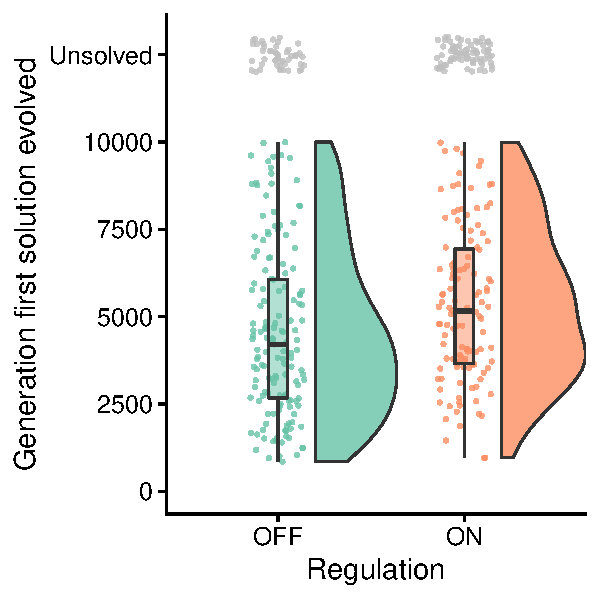
\includegraphics[width=\textwidth]{chapters/05-tag-based-genetic-regulation/media/boolean-calc-postfix-solve-time-cloud.pdf}
    \caption{\small Generations elapsed before solution.}
    \label{chapter:tag-based-regulation:subfig:boolean-calc-postfix-solve-time}
\end{subfigure}

\caption{\small 
\textbf{Boolean-logic calculator (postfix notation)  problem-solving performance.}
(a) shows the number of successful replicates for the regulation-off and regulation-on conditions on the postfix Boolean-logic calculator problem. 
The regulation-on condition was less successful than the regulation-off condition (Fisher's exact test: $p<0.002$).
(b) is a Raincloud plot showing the generation at which the first solution evolved in each successful replicate.
Gray points indicate the unsuccessful replicates for each condition.
Regulation-off solutions typically required fewer generations than regulation-on solutions to arise (Wilcoxon rank sum test: $p<0.004$).
}
% fisher's exact: p-value = 0.001286
% wilcoxon:  p-value = 0.003285
\label{chapter:tag-based-regulation:fig:boolean-calc-postfix-performance}
\end{figure}
